\textbf{Motivation}: So far, when looking for $\hat{f}(x)$ the form was $\hat{f}(x)=w^\top x$, or $\hat{f}(x) = w^\top \phi(x)$. 
Note how the features $x, \phi(x)$ are predetermined. Why not learn them?

\textbf{New Optimization Problem}:

The new join-optimization problem, for $w$ and $\phi$:\\
\subtext{$\Theta$ is a set of parameters for $\phi$}
$$
    \hat{w} = \underset{w\in\R^m,\Theta\in\R^{m\times d}}{\text{arg min}}\Biggl( \frac{1}{n}\sum_{i=1}^n l\Bigl( w^\top \phi(x_i;\Theta),y_i \Bigr) \Biggr)
$$
Where $\phi(x,\Theta) = \Bigl( \phi_1(x;\theta_1),\ldots,\phi_m(x;\theta_m) \Bigr)$.\\
\subtext{$\theta_i$ is the $i$th row of $\Theta$, i.e. $\theta_i := (\Theta)_{i,:}$}

More compact, in terms of $\Theta$, which combines $w, \phi$:
$$
    \Theta^* := \underset{\Theta}{\text{arg min}}\Bigl( L(\Theta; \mathcal{D}) \Bigr) = \underset{\Theta}{\text{arg min}} \Biggl( \frac{1}{n} \sum_{i=1}^{n} l\Bigl( \Theta;x_i,y_i \Bigr) \Biggr)
$$
\subtext{$\Theta$ may also encapsulate $w,\phi$ for multiple layers, depending on definition}

\subsection{Definitions}

\definition \textbf{Activation Function}\\
We set $\phi_i(x;\theta_i) = \psi(\theta_i^\top x)$, $\psi$ is the activation function.\\
\subtext{$\theta_i \in \R^d,\quad\psi:\R\to\R$}

{\scriptsize
    \notation More concisely, $\phi(x;\Theta) = \psi(\Theta x)$
}

\begin{center}
    \begin{tabular}{ll}
        \textbf{Activation Function}    & \textbf{Definition}               \\
        \hline
        Identity                        & $\psi(z) = z$                     \\
        Sigmoid                         & $\psi(z) = \frac{1}{1+e^{-z}}$    \\
        Hyperbolic tangent              & $\psi(z) = \tanh(z)$              \\
        Rectified Linear Unit (ReLU)    & $\psi(z) = \max(0,z)$ 
    \end{tabular}
\end{center}

\definition \textbf{Artificial Neural Network}\\
\subtext{The output functions of the above problem take the form:}
$$
    f(x;w,\theta) = \sum_{j=1}^{m}w_j\psi(\theta_j^\top x)
$$
{\scriptsize
    \remark Also called Multi-Layer Perceptron (MLP)
}

\newpage
\textbf{What is happening here?}\\
\smalltext{Explaining the calculation steps for such an $f$ naturally leads to the common pictorial depiction of neural networks.}
\begin{align*}
    \text{(i)}      &\quad x       &=\quad& (x_1,\ldots,x_n) \in \R^d       & \text{(Input Vector)}             \\
    \text{(ii)}     &\quad z       &=\quad& \Theta x                        & \text{(Linear transformation)}    \\
    \text{(iii)}    &\quad h_i     &=\quad& \psi(z_i)                       & \text{(Activation function)}      \\
    \text{(iv)}     &\quad f(x)    &=\quad& \sum_{j=1}^m w_j h_j            & \text{(Output)}
\end{align*}

\definition \textbf{Hidden Layer} $h = \psi(z)$

\definition \textbf{Bias Term} $b \in \R^m$\\
\subtext{Needed, as $f$ might not pass through origin. Similar to using $F_\text{lin}$ in regression, these can also be added by augmenting the input \& hidden layers.}

\textbf{Does this work at all?}\\
\smalltext{Yes, for most functions this does work.}

\definition \textbf{Sigmoidal Function}
$$
    \sigma(t) \text{ s.t. } \begin{cases}
        \sigma: \R \to \R \\
        \underset{t\to\infty}{\lim} = 1 \text{ and } \underset{t\to\infty}{\lim}
    \end{cases}
$$

\theorem \textbf{Universal Approximation Theorem}\\
\smalltext{$\hat{f}$, that uniformly approximates $f$, exists and takes this form:}
$$
    \hat{f}(x) = \textbf{W}^{(2)}\psi\Bigl( \textbf{W}^{(1)}x + b \Bigr)
$$ 
\smalltext{$f: [0,1]^d\to\R$ continuous$,\quad \psi $ sigmoidal}\\
\subtext{$\textbf{W}^{(1)} \in\R^{m\times d},\quad \textbf{W}^{(2)}\in\R^{1\times m},\quad m \in \N$}

Note how $m$ could be very large.\\
\subtext{$m$ can intuitively be understood as the "width" of the ANN}

\newpage
\definition \textbf{Fully Connected Neural Network}

More complex ANNs might have:
\begin{enumerate}
    \item More hidden layers
    \item Multiple outputs
    \item Differen activation functions across layers
\end{enumerate}
These are called \textit{fully connected}, since every node in a layer is connected to every node in the adjacent layers.\\
\subtext{There are also more complex architectures.}
\begin{center}
    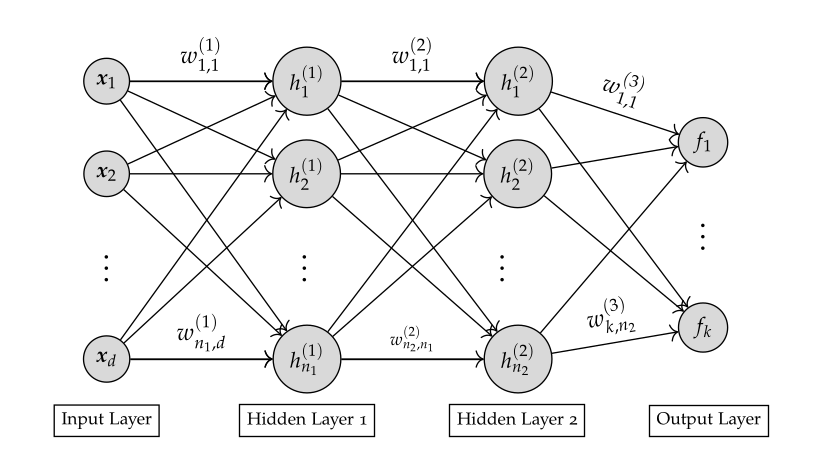
\includegraphics[width=0.9\linewidth]{resources/FCANN.png}\\
    \subtext{\textit{Introduction to Machine Learning (2026), p. 183}}
\end{center}

\notation Weights: $\textbf{W}^{(i)} := \Bigl[ w_{k,l}^{(i)} \Bigr]$, Biases: $b^{(i)}_k$\\
and $\Theta = \Bigl(\textbf{W}^{(1)},\ldots,\textbf{W}^{(L)}, b^{(1)},\ldots,b^{(L)}\Bigr)$ (All parameters)\\
\subtext{$w_{k,l}^{(i)}$: "Weight at layer $i$ to node $k$ from node $l$"} 

\newpage
\subsection{Forward Propagation}


How can we make predictions, i.e. how can $\hat{f}$ be evaluated?

\definition \textbf{Forward Propagation}\\
\subtext{This is just the computation for $1$-layer ANN generalized for $L$ layers}


\begin{algorithm}
    \caption{Forward Propagation}
    $h^{(0)}\gets x$\;
    \For{$l=1,\ldots,L$}{
        $z^{(l)} = \textbf{W}^{(l)}h^{(l-1)} + b^{(l)}$ \\
        $h^{(l)} = \psi(z^{(l)})$
    }
    $f \gets \textbf{W}^{(L)}h^{(L-1)}+b^{(L)}$ \\
    \Return f
\end{algorithm}

\subsection{Backwards Propagation}

How can we get all gradients needed for model training?

\definition \textbf{Backwards Propagation}

\textbf{Intuition}: An efficient way to get the gradients is to reuse results from forward prop. and previous steps. This works best when starting at the back, at $\nabla_{\textbf{W}^{(L)}}l$.

\textbf{Goal}: $\nabla_{\textbf{W}^{(1)}}l,\ldots,\nabla_{\textbf{W}^{(L)}} l, \nabla_{b^{(1)}}l,\ldots,\nabla_{b^{(L)}}l$

\textbf{Step 1}: Calculate $\nabla_{\textbf{W}^{(L)}}l$, i.e. start from the back.
\begin{align*}
    \nabla_{\textbf{W}^{(L)}}l  &= \frac{\partial l}{\partial \textbf{W}^{L}} \\
                                &= \frac{\partial l}{\partial f}\cdot\frac{\partial f}{\partial \textbf{W}^{(L)}} & \text{(Chain Rule)} \\
                                &= \frac{\partial l}{\partial f}\cdot\begin{bmatrix}
                                    \bigl( h^{(L-1)} \bigr)^\top    \\
                                    \vdots                          \\
                                    \bigl( h^{(L-1)} \bigr)^\top    
                                \end{bmatrix}                                                                     & (f = \textbf{W}^{(L)}h^{(L-1)} + b^{(L)}) \\
                                &= \nabla_f l \cdot\begin{bmatrix}
                                    \bigl( h^{(L-1)} \bigr)^\top    \\
                                    \vdots                          \\
                                    \bigl( h^{(L-1)} \bigr)^\top    
                                \end{bmatrix}                                                                     & \Biggl(\frac{\partial l}{\partial f} = \nabla_f l\Biggr)
\end{align*}
Notice how $h^{(L-1)}$ was computed during forward prop.

\newpage

\textbf{Step 2}: Calculate $\nabla_{\textbf{W}^{(L-1)}}l$.
\begin{align*}
    \nabla_{\textbf{W}^{(L-1)}}l    &= \underbrace{\frac{\partial l}{\partial f}}_{\text{(1)}}\cdot\underbrace{\frac{\partial f}{\partial h^{(L-1)}}}_{\text{(2)}}\cdot\underbrace{\frac{\partial h^{(L-1)}}{\partial z^{(L-1)}}}_\text{(3)}\cdot\underbrace{\frac{z^{(L-1)}}{\partial \textbf{W}^{(L-1)}}}_\text{(4)}      & \text{(Chain Rule)} \\
\end{align*}
\begin{enumerate}
    \item Already done in Step 1.
    \item Already done in forward propagation, equal to $\textbf{W}^{(L)}$:
    $$
        f \overset{\text{def}}{=} \textbf{W}^{(L)}h^{(L-1)}+b^{(L)} \implies \frac{\partial f}{\partial h^{(L-1)}} = \textbf{W}^{(L)}
    $$
    \item \textbf{Not done.} Needs to be calculated:
    \begin{align*}
        \frac{\partial h^{(L-1)}}{\partial z^{(L-1)}}   &= \frac{\partial \psi\bigl( z^{(L-1)} \bigr)}{\partial z^{(L-1)}}  \\
                                                        &= \text{diag}\Bigl( \psi'\bigl( z^{(L-1)} \bigr) \Bigr)            \\
                                                        &= \begin{bmatrix}
                                                            \psi'\Bigl(z_1^{(L-1)}\Bigr) & 0 & \cdots & 0 \\
                                                            0 & \psi'\Bigl(z_2^{(L-1)}\Bigr) & \cdots & 0 \\
                                                            \vdots & \vdots & \ddots & \vdots             \\
                                                            0 & 0 & \cdots & \psi\Bigl(z_n^{(L-1)}\Bigr)  \\
                                                        \end{bmatrix}  
    \end{align*}
    \item Already done in forward propagation, analogous to step 1. 
    $$
        \frac{\partial z^{(L-1)}}{\partial \textbf{W}^{(L-1)}} =
        \begin{bmatrix}
            \bigl( h^{(L-2)} \bigr)^\top    \\
            \vdots                          \\
            \bigl( h^{(L-2)} \bigr)^\top
        \end{bmatrix}
    $$
\end{enumerate}

\textbf{Step $i \leq L$}: Calculate $\nabla_{\textbf{W}^{(L-i)}}l$ Analogoues to step 2.\\
\subtext{The biases $\nabla_{b^{(l)}}l$ are analogous.}

\newpage

\subsection{Optimization}

\textbf{Problem}: How can we train the model, i.e find $\Theta^*$?
$$
    \Theta^* := \underset{\Theta}{\text{arg min}}\Bigl( L(\Theta; \mathcal{D}) \Bigr) = \underset{\Theta}{\text{arg min}} \Biggl( \frac{1}{n} \sum_{i=1}^{n} l\Bigl( \Theta;x_i,y_i \Bigr) \Biggr)
$$

{\footnotesize
    \remark $L(\Theta;\mathcal{D})$ is generally not convex.\\
    {\color{gray}
        i.e. local minima, saddle points may exist
    }

    \remark $\dim(\Theta)$ is the total param. count of NN, may be very large
}

\textbf{Solution}: Gradient Descent (with optimizations)
\begin{itemize}
    \item Stochastic Gradient Descent\\
    \subtext{(Why? $\dim(\Theta)$ is very large, $\nabla_\Theta l(\Theta;x_i,y_i)$ are expensive)}
    \item Minibatch Gradient Descent\\
    \subtext{(Why? $\mathcal{D}$ may be very large, so there are \textit{many} gradients)}
\end{itemize}

The standard GD update for $\Theta$ is:
$$
    \Theta^{t+1} = \Theta^t - \eta_t\cdot\nabla_\Theta L\Bigl( \Theta;\mathcal{D} \Bigr)
$$
In Minibatch GD, this becomes:\\
\subtext{Where $\mathcal{S} \subset \{1,\ldots,n\}$}
$$
    \Theta^{t+1} = \Theta^t - \eta_t\cdot\nabla_\Theta L\Biggl( \frac{1}{|\mathcal{S}|}\sum_{i\in \mathcal{S}} l\Bigl( \Theta^t; x_i,y_i \Bigr) \Biggr)
$$

{\footnotesize
    \remark An advantage: If $\Theta^t$ approaches a stationary point (which isn't the global minimu), GD will converge, but MB-GD may not converge.
}